%!  pour pdfLatex
\documentclass[a4paper]{article}
%\usepackage[hmargin={1.5cm,1.5cm},vmargin={2.4cm,2.4cm},headheight=13.1pt]{geometry}
\usepackage[a4paper,landscape,twocolumn,
            hmargin=1.8cm,vmargin=2.2cm,headheight=13.1pt]{geometry}

\usepackage[pdftex]{graphicx,color}
\usepackage[pdftex,colorlinks={true},urlcolor={blue},pdfauthor={remy Nicolai}]{hyperref}

\usepackage[T1]{fontenc}
\usepackage[utf8]{inputenc}

\usepackage{lmodern}
\usepackage[frenchb]{babel}

\usepackage{fancyhdr}
\pagestyle{fancy}

\usepackage{floatflt}
\usepackage{maths}

\usepackage{parcolumns}
\setlength{\parindent}{0pt}

\usepackage{caption}
\usepackage{subcaption}

\usepackage{makeidx}

\usepackage[french,ruled,vlined]{algorithm2e}
\SetKwComment{Comment}{\#}{}
\SetKwFor{Tq}{tant que}{}{}
\SetKwFor{Pour}{pour}{}{}
\DontPrintSemicolon
\SetAlgoLined

\usepackage{listings}
\lstset{language=Python,frame=single}
\lstset{literate=
  {á}{{\'a}}1 {é}{{\'e}}1 {í}{{\'i}}1 {ó}{{\'o}}1 {ú}{{\'u}}1
  {Á}{{\'A}}1 {É}{{\'E}}1 {Í}{{\'I}}1 {Ó}{{\'O}}1 {Ú}{{\'U}}1
  {à}{{\`a}}1 {è}{{\`e}}1 {ì}{{\`i}}1 {ò}{{\`o}}1 {ù}{{\`u}}1
  {À}{{\`A}}1 {È}{{\'E}}1 {Ì}{{\`I}}1 {Ò}{{\`O}}1 {Ù}{{\`U}}1
  {ä}{{\"a}}1 {ë}{{\"e}}1 {ï}{{\"i}}1 {ö}{{\"o}}1 {ü}{{\"u}}1
  {Ä}{{\"A}}1 {Ë}{{\"E}}1 {Ï}{{\"I}}1 {Ö}{{\"O}}1 {Ü}{{\"U}}1
  {â}{{\^a}}1 {ê}{{\^e}}1 {î}{{\^i}}1 {ô}{{\^o}}1 {û}{{\^u}}1
  {Â}{{\^A}}1 {Ê}{{\^E}}1 {Î}{{\^I}}1 {Ô}{{\^O}}1 {Û}{{\^U}}1
  {œ}{{\oe}}1 {Œ}{{\OE}}1 {æ}{{\ae}}1 {Æ}{{\AE}}1 {ß}{{\ss}}1
  {ű}{{\H{u}}}1 {Ű}{{\H{U}}}1 {ő}{{\H{o}}}1 {Ő}{{\H{O}}}1
  {ç}{{\c c}}1 {Ç}{{\c C}}1 {ø}{{\o}}1 {å}{{\r a}}1 {Å}{{\r A}}1
  {€}{{\euro}}1 {£}{{\pounds}}1 {«}{{\guillemotleft}}1
  {»}{{\guillemotright}}1 {ñ}{{\~n}}1 {Ñ}{{\~N}}1 {¿}{{?`}}1
}

%pr{\'e}sentation des compteurs de section, ...
\makeatletter
\renewcommand{\thesection}{\Roman{section}.}
\renewcommand{\thesubsection}{\arabic{subsection}.}
\renewcommand{\thesubsubsection}{\arabic{subsubsection}.}
\renewcommand{\labelenumii}{\theenumii.}
\makeatother


\newtheorem*{thm}{Théorème}
\newtheorem{thmn}{Théorème}
\newtheorem*{prop}{Proposition}
\newtheorem{propn}{Proposition}
\newtheorem*{pa}{Présentation axiomatique}
\newtheorem*{propdef}{Proposition - Définition}
\newtheorem*{lem}{Lemme}
\newtheorem{lemn}{Lemme}

\theoremstyle{definition}
\newtheorem*{defi}{Définition}
\newtheorem*{nota}{Notation}
\newtheorem*{exple}{Exemple}
\newtheorem*{exples}{Exemples}


\newenvironment{demo}{\renewcommand{\proofname}{Preuve}\begin{proof}}{\end{proof}}
%\renewcommand{\proofname}{Preuve} doit etre après le begin{document} pour fonctionner

\theoremstyle{remark}
\newtheorem*{rem}{Remarque}
\newtheorem*{rems}{Remarques}

%\usepackage{maths}
%\newcommand{\dbf}{\leftrightarrows}

%En tete et pied de page
\lhead{Informatique}
%\chead{Introduction aux systèmes informatiques}
\rhead{MPSI B Hoche}
\lfoot{\tiny{Cette création est mise à disposition selon le Contrat\\ Paternité-Partage des Conditions Initiales à l'Identique 2.0 France\\ disponible en ligne http://creativecommons.org/licenses/by-sa/2.0/fr/  
} 
\rfoot{\tiny{Rémy Nicolai \jobname \; \today } }
}
\makeindex

\begin{document}
\chead{TP 3 (14/10 et 04/11 2013)}
Toute écriture d'une fonction en Python doit être PR\'EC\'ED\'EE par une implémentation en pseudo-code.
\subsection{Boustrophédon}
Une écriture de type \emph{boustrophédon} traite ses lignes alternativement dans un sens et dans l'autre. Le premier tableau indique la place où s'écrivent sur 4 lignes de 4 caractères les 16 caractères d'un texte. Le second présente le début de cet énoncé en écriture boustrophédon sur des lignes de 10 caractères
\begin{center}
\begin{tabular}{l|cccc}
ligne 1 & 1 & 2 & 3 & 4\\
ligne 2 & 8 & 7 & 6 & 5\\
ligne 3 & 9 & 10 & 11 & 12\\
ligne 4 & 16 & 15 & 14 & 13
\end{tabular}
\hfill
\begin{tabular}{cccccccccc}
 U & n & e &   & é & c & r & i & t & u \\
 e & p & y & t &   & e & d &   & e & r \\
   & b & o & u & s & t & r & o & p &  h \\
 t & i & a & r & t &   & n & o & d & é  \\
 e &   & s & e & s &   & l & i & g & n 
 \end{tabular}
\end{center}

\begin{enumerate}
 \item 
\begin{enumerate}
 \item Former une fonction nommée \verb|tronq| qui prend deux paramètres \verb|texte| et \verb|L| tels que la longueur de la chaîne de caractères désignée par \verb|texte| soit supérieure ou égale au nombre entier désigné par \verb|L| et renvoie la chaîne tronquée aux $L$ premiers caractères.\newline
 Former une fonction nommée \verb|compl| qui prend deux paramètres \verb|texte| et \verb|L| tels que la longueur de la chaîne de caractères soit strictement inférieure à $L$ et renvoie la chaîne complétée par des caractères " " (espace). 

 \item  Former une fonction nommée \verb|boustro1| prenant trois paramètres \verb|texte|, \verb|p|, \verb|q| (désignant respectivement une chaîne de caractères et deux entiers strictement plus grands que 1) et renvoyant une liste de $q$ chaînes de $p$ caractères. Si le texte contient plus de $pq$ caractères, il sera tronqué aux $pq$ premiers. si le texte contient moins de $pq$ caractères, on le complète par des espaces. Cette fonction utilisera les fonctions \verb|tronq| et \verb|compl|. 

 \item Cherchez ce qu'est un \og Lorem Ipsum \fg \ et récupérez le Lorem Ipsum standard. Affichez le en écriture boustrophédon sur 10 lignes de 30 caractères.
 \end{enumerate}

\item On considère $\N \times \Z$ présenté comme un tableau avec des lignes indexées par un élément de $\N$ et des colonnes par un élément de $\Z$. Dans cet ensemble, une partie $\mathcal{E}$ est définie comme sur la figure \ref{fig:Eboustro_1}. Elle s'étend indéfiniment vers le bas et on numérote ses éléments comme pour une écriture de type boustrophédon (figure \ref{fig:Eboustro_2}).

\begin{figure}
  \centering
  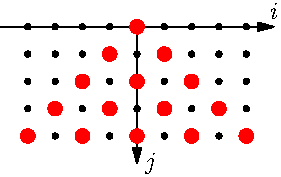
\includegraphics{./Eboustro_1_fig.pdf}
  \caption{Partie $\mathcal{E}$.}
  \label{fig:Eboustro_1}
\end{figure}

\begin{figure}
  \centering
  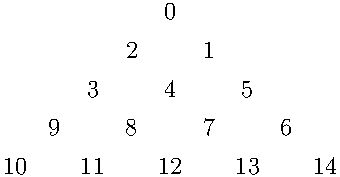
\includegraphics{./Eboustro_2_fig.pdf}
  \caption{Numérotation et ordre}
  \label{fig:Eboustro_2}
\end{figure}
On associe à chaque point de $\mathcal{E}$ un nombre que l'on forme par un procédé analogue à celui du triangle de Pascal avec les règles suivantes (voir figure \ref{fig:Eboustro_3}) .
\begin{itemize}
  \item Le nombre $1$ est associé au point $(0,0)$ de numéro $0$.
  \item Les lignes sont parcourues alternativement d'un côté à  l'autre. Le premier élément d'une nouvelle ligne reçoit toujours $0$.
  \item Le nombre associé à un point d'une ligne est la somme des nombres associés au point précédent et au point de la ligne du dessus.
\end{itemize}
\begin{figure}
  \centering
  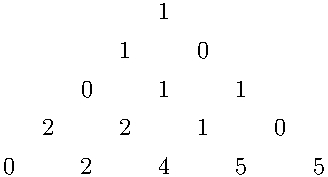
\includegraphics{./Eboustro_3_fig.pdf}
  \caption{Nombres associés aux points de $\mathcal{E}$.}
  \label{fig:Eboustro_3}
\end{figure}
\begin{enumerate}
  \item Soit $(i,j)\in \Z \times \N$. Caractériser par des propriétés de $i+j$ et $i-j$ le fait que $(i,j)\in \mathcal{E}$.
  \item Calculer mathématiquement le numéro d'un point $(i,j)\in \mathcal{E}$.
  \item Former une fonction nommée \verb|suivant| qui prend deux paramètres \verb|i| et \verb|j| désignant respectivement des éléments $i$ de $\Z$ et  $j$ de $\N$ tels que $(i,j)\in \mathcal{E}$ et qui renvoie le tuple des deux coordonnées du point suivant de $\mathcal{E}$ pour l'ordre choisi.
  \item Former une fonction nommée \verb|num| qui prend deux paramètres \verb|i| et \verb|j| désignant respectivement des éléments $i$ de $\Z$ et  $j$ de $\N$ et qui renvoie le numéro du point $(i,j)$ s'il appartient à $\mathcal{E}$ et $-1$ s'il n'y appartient pas. Cette fonction devra utiliser la fonction \verb|suivant| et non l'expression mathématique.
  \item Former une fonction nommée \verb|boustro2| qui prend un paramètre \verb|n| désignant un entier naturel $n$ et qui renvoie un dictionnaire (indexé par les tuples de coordonnées) des valeurs associées aux $n$ premiers points de $\mathcal{E}$. On pourra utiliser une liste contenant les deux coordonnées d'un point ainsi que le sens de parcours (codé par $+1$ pour gauche-droite et $-1$ pour droite-gauche) au point représenté. 
\end{enumerate}

\end{enumerate}

\subsection{Palindromes}
Un palindrome\footnote{ "Tu l'as trop écrasé, César, ce Port-Salut ! " (alexandrin attribué à Victor Hugo)} est un mot ou une phrase qui se lit dans les deux sens. Un \emph{nombre entier sera dit palindrome}\footnote{\href{http://fr.wikipedia.org/wiki/Nombre\_palindrome}{http://fr.wikipedia.org/wiki/Nombre\_palindrome}} lorsque son écriture décimale est un palindrome de chiffres (comme 141 par exemple).

\subsubsection{Retournement d'une liste}
Former en Python une procédure nommée \verb|retournL| qui prend un paramètre \verb|L| désignant une \emph{liste} et le modifie en le renversant. La procédure de renverra rien.\newline
En Python, les objets du type liste possèdent une méthode \verb|reverse()| qui a le même effet, vous pouvez l'utiliser dans la suite à la place de la fonction que vous avez écrite car elle est vraisemblablement plus efficace.

\subsubsection{Décomposition et composition}
\begin{enumerate}
  \item Former une fonction nommée \verb|decomp| qui prend un paramètre \verb|n| désignant un nombre entier et qui renvoie la liste écrite dans le sens habituel des chiffres de son écriture décimale.
  \item Le nom \verb|L| désignant une liste de nombres entre $0$ et $9$ (indexée à partir de $0$), on considère les algorithmes représentés par les pseudo-codes suivants \newline
Algorithme I (naïf)
  \begin{itemize}
    \item \verb|i| $\longleftarrow$ (longueur de \verb|L|) $-1$
    \item \verb|v| $\longleftarrow 0$
    \item pour $c$ décrivant les valeurs de \verb|L| en partant du plus grand index
    \begin{itemize}
      \item \verb|v| $\longleftarrow v + c* 10^i$
      \item décrémenter \verb|i|
    \end{itemize}
    \item renvoyer \verb|v|
  \end{itemize}
Algorithme II (Hörner)
\begin{itemize}
  \item \verb|v| $\longleftarrow 0$
  \item \verb|i| $\longleftarrow 0$
  \item tant que \verb|i < longueur(L)|
  \begin{itemize}
    \item \verb|v| $\longleftarrow$ \verb|10*v + L[i]|
    \item incrémenter \verb|i|
  \end{itemize}
  \item renvoyer \verb|v|
\end{itemize}
\begin{enumerate}
  \item Montrer que les deux algorithmes renvoient le même nombre. Pour une chaîne de longueur $n$, calculer le nombres d'additions et de multiplications effectuées par chaque algorithme.
  \item Former une fonction nommée \verb|comp| qui prend un paramètre $L$ et qui renvoie le nombre dont cette liste est l'écriture décimale habituelle. 
\end{enumerate}
\end{enumerate}

\subsubsection{Retournement d'un nombre}
Pour tout entier naturel $n$, on désigne par $\overleftarrow{n}$ le nombre dont le développement décimal est obtenu en retournant la liste du développement de $n$. Par exemple, si $n = 2453$ alors $\overleftarrow{n}=3542$.\newline
Pour tout nombre entier $n$, on considère la suite $\left( n_i \right)_{i\in\N}$ définie par $n_0 = n$ et 
\begin{displaymath}
  \forall i\in \N : n_{i+1} = n_i + \overleftarrow{n_i}
\end{displaymath}
Il semblerait (conjecture) que, pour tout $n$, il existe un $i$ tel que $n_i$ soit un nombre palindrome. Lorsqu'il existe de tels $i$, on note $\delta(n)$ le plus petit d'entre eux. Lorsqu'il n'existe pas un tel $i$ le nombre $n$ est dit \emph{de Lychrel}. On ne connait pas de nombre de Lychrel mais on ne sait pas non plus montrer qu'il n'en existe pas.
\begin{enumerate}
\item \'Ecrire une fonction nommée \verb|retournN| qui prend un paramètre \verb|n| désignant un entier naturel $n$ et qui renvoie $\overleftarrow{n}$ puis une fonction \verb|sym| qui renvoie $n+\overleftarrow{n}$.
\item 
\begin{enumerate}
 \item Former une fonction \verb|delta(n,p)| qui renvoie $\delta(n)$ lorsque $\delta(n)\leq p$. 
 \item Déterminer les deux plus petits nombres dont vous ne savez pas montrer qu'ils ne sont pas de Lychrel.
\end{enumerate}
\end{enumerate}

\end{document}
